% !TeX spellcheck = pl_PL 
\chapter{Specyfikacja zewnętrzna}
\section{Wymagania sprzętowe}
Aplikacja działa pod systemami Windows 7 i nowszymi, na architekturze 64-bitowej. Instalacja nie jest wymagana, wystarczy otworzyć plik aplikacji .exe by móc z niej korzystać. Wszystkie biblioteki i pliki konfiguracyjne nie mogą zostać zmienione.
\section{Korzystanie z aplikacji}
Po uruchomieniu programu pojawia się okno z interfejsem graficznym złożonym z kilku podstawowych sekcji.
\begin{figure}[H]
	\centering
	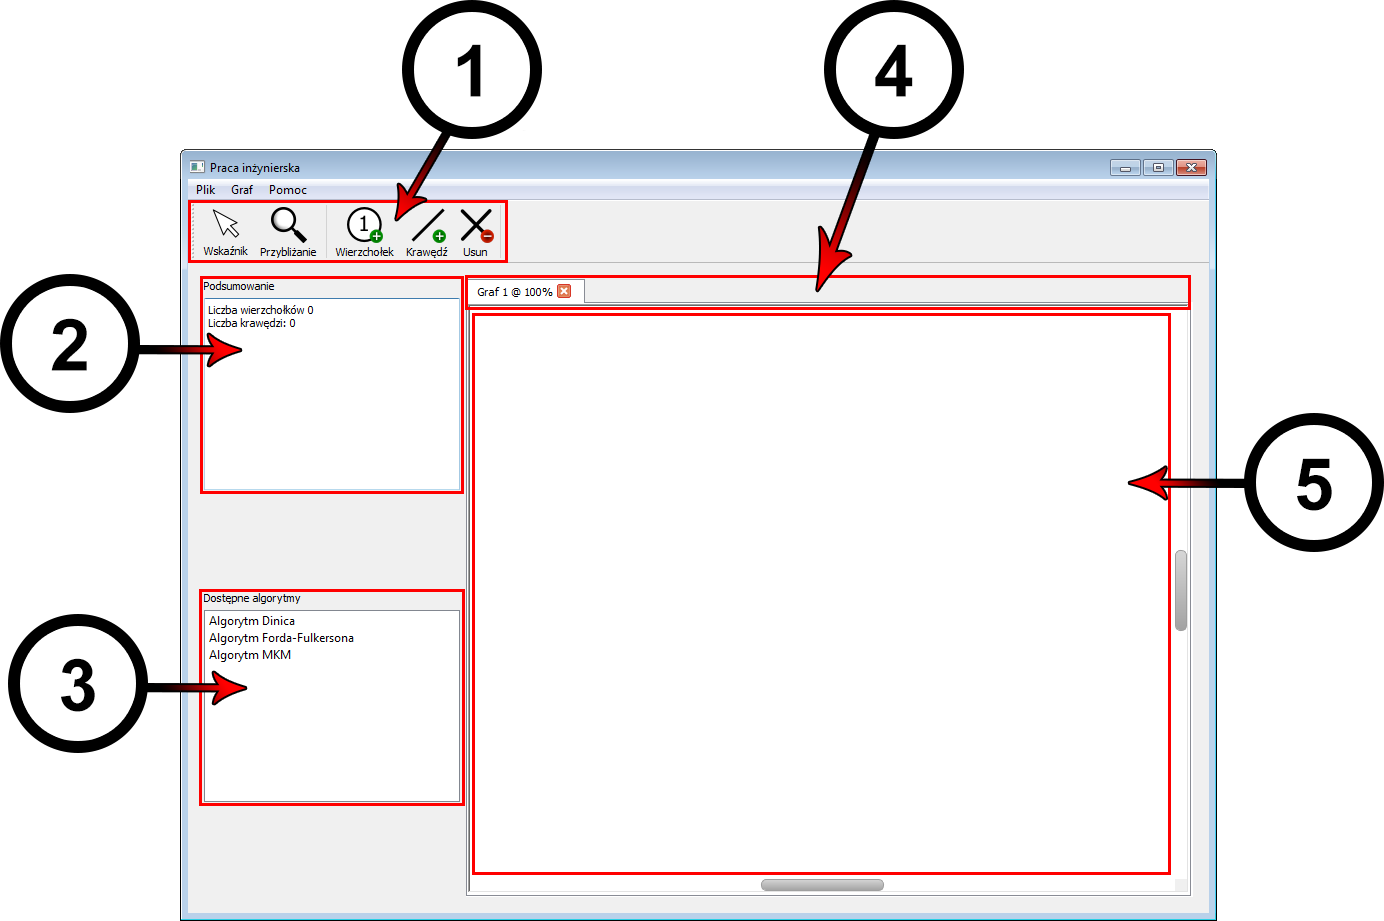
\includegraphics[width=0.85\textwidth]{./img/spec_zew01-1.png}
	\caption{Interfejs graficzny}
\end{figure}
\begin{enumerate}
	\item \textit{Pasek narzędziowy} obejmuje pięć narzędzi do pracy z siecią przepływową: wskaźnik, lupę, dodanie grafu, dodanie krawędzi i usunięcie elementu.
	\item \textit{Podsumowanie} zawiera informacje na temat aktywnej w danej chwili sieci.
	\item \textit{Dostępne algorytmy} zawierają listę operacji, jakie można na sieci wykonać.
	\item \textit{Pasek kart} zawiera listę istniejących sieci w instancji aplikacji między którymi można się przełączać.
	\item \textit{Pole edycji grafu} to miejsce robocze, gdzie można umieszczać elementy grafu i pracować nad nim.
\end{enumerate}
\subsection{Tworzenie nowej sieci}
Aby utworzyć nową sieć należy z paska menu wybrać \menu{Plik > Nowy} lub skorzystać ze skrótu \keys{\ctrl + N}. Następnie pojawi się okienko w które należy wpisać roboczą nazwę sieci (można też pozostawić wygenerowaną domyślną nazwę). Po zatwierdzeniu zostanie dodana nowa karta z pustym polem edycyjnym.
\begin{figure}[H]
	\centering
	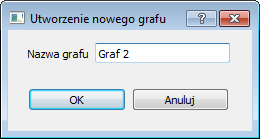
\includegraphics[width=0.3\textwidth]{./img/spec_zew02}
	\label{fig:nowyGrafMsgbox}
	\caption{Okienko z wyborem nazwy}
\end{figure}
\subsection{Rysowanie grafu}
\subsubsection{Dodanie wierzchołka}
Aby dodać nowy wierzchołek należy wybrać narzędzie dodawania wierzchołków, a następnie kliknąć lewym przyciskiem myszy na puste miejsce w polu edycyjnym. Pojawi się nowy obiekt, miejsce kliknięcia będzie środkiem wierzchołka. Jeżeli klikniemy istniejący już obiekt, zostanie on zaznaczony.
\subsubsection{Dodanie łuku}
Aby móc dodać łuk na polu roboczym muszą istnieć co najmniej dwa wierzchołki. Należy wybrać narzędzie dodawania krawędzi i w pierwszej kolejności kliknąć na wierzchołek który będzie źródłem. Pojawi się nad nim etykieta \textit{"Źródło"}. Potem należy kliknąć drugi wierzchołek, po najechaniu myszką pojawi się nad nim etykieta \textit{"Ujście"}. Kliknięcie lewym przyciskiem myszy spowoduje potwierdzenie operacji i pojawienie okienka, gdzie należy wpisać przepływ i przepustowość tego łuku, domyślnie zero i jeden. Jeżeli między wierzchołkami już istnieje dane połączenie, operacja zostanie zignorowana. Łuk jest na trwał e przymocowany do wierzchołków i nie można zmienić jego pozycji. Etykieta zawiera informację w formacie \emph{"przepływ / przepustowość"}.
\begin{figure}[h]
	\centering
	\begin{subfigure}{0.28\textwidth}
		\caption{}
		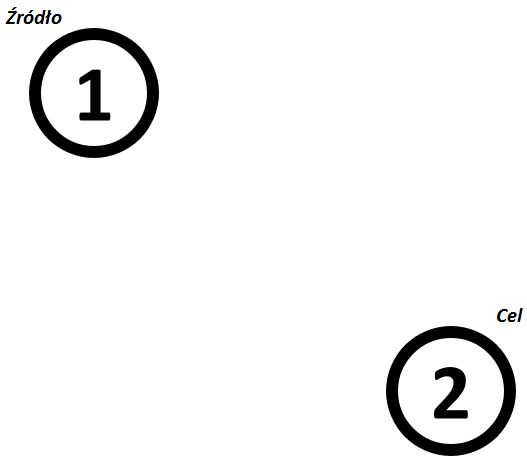
\includegraphics[width=0.9\linewidth]{./img/spec_zew03_1.png}
		\label{fig:addEdge1}
	\end{subfigure}\hfill
	\begin{subfigure}{0.28\textwidth}
		\caption{}
		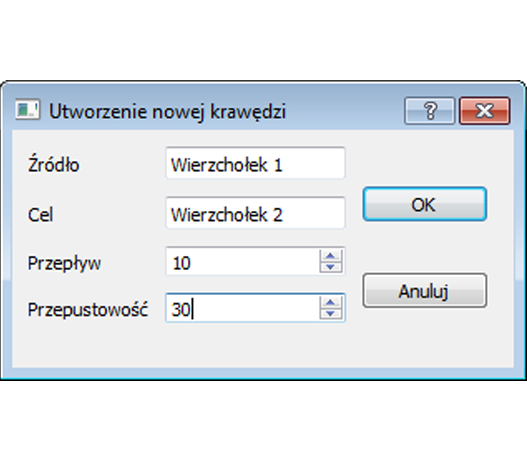
\includegraphics[width=0.9\linewidth]{./img/spec_zew03_2.png}
		\label{fig:addEdge2}
	\end{subfigure}\hfill
	\begin{subfigure}{0.28\textwidth}
		\caption{}
		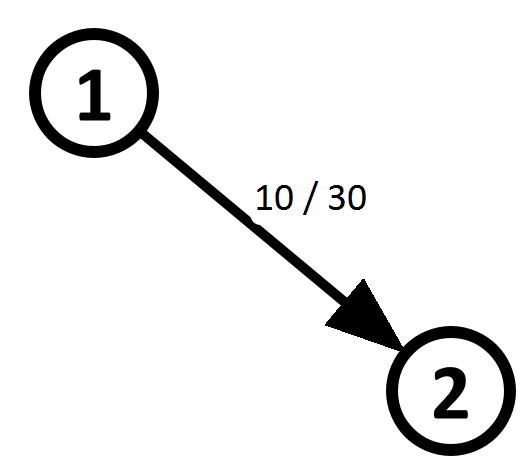
\includegraphics[width=0.9\linewidth]{./img/spec_zew03_3.png}
		\label{fig:addEdge3}
	\end{subfigure}
	\caption{Etapy dodawania łuku}
	\label{fig:addEdge}
\end{figure}
\subsubsection{Usuwanie elementów}
W każdej chwili można usunąć wierzchołek lub łuk w sieci. W tym celu należy wybrać narzędzie usuwania oraz kliknąć wybrany element. Usunięcie łuku powoduje pozbycie się z sieci tylko niego, z kolei usunięcie wierzchołka powoduje zlikwidowanie wszystkich łuków, które wchodzą lub wychodzą z niego. Można usuwać wiele elementów naraz, narzędzie usuwa wszystko co jest zaznaczone. 
\subsubsection{Poprawa estetyki sieci}
Aby poprawić wygląd i czytelność sieci istnieje możliwość wyrównania pozycji wierzchołków. Wszystkie wierzchołki w sieci posiadają te same rozmiary i dzięki temu można zastosować kilka sposobów ich wyrównania. W tym celu należy zaznaczać dwa lub więcej wierzchołków, a następnie kliknąć jedną z kombinacji klawiszy:
\begin{itemize}
	\item \keys{\shift + \arrowkeyup} - ustawia pozycję pionową wszystkich wierzchołków równą pozycji wierzchołka najbardziej wysuniętego do góry.
	\item \keys{\shift + \arrowkeydown} - ustawia pozycję pionową wszystkich wierzchołków równą pozycji wierzchołka najbardziej wysuniętego na dół.
	\item \keys{\shift + \arrowkeyleft} - ustawia pozycję poziomą wszystkich wierzchołków równą pozycji wierzchołka najbardziej wysuniętego na lewo.
	\item \keys{\shift + \arrowkeyright} - ustawia pozycję poziomą wszystkich wierzchołków równą pozycji wierzchołka najbardziej wysuniętego na prawo.
\end{itemize}
\subsubsection{Konfiguracja wyglądu grafu}
Rozmiar i kolory wierzchołków oraz łuków można modyfikować w ustawieniach. W tym celu należy wybrać z paska menu \menu{Graf > Kształt} lub skorzystać ze skrótu klawiszowego \menu{\ctrl + \shift + K}. Pojawi się okienko z konfiguracją lokalnego grafu.
\begin{figure}[H]
	\centering
	\begin{subfigure}{0.45\textwidth}
		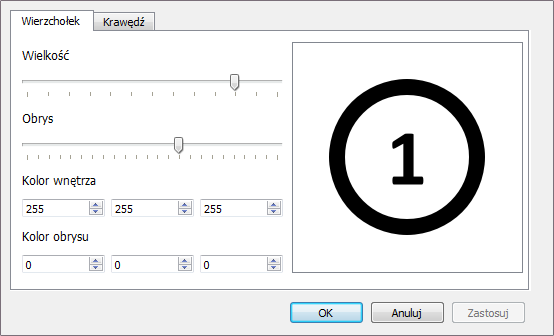
\includegraphics[width=0.9\linewidth]{./img/spec_zew04_1.png}
		\caption{Konfiguracja wierzchołków}
		\label{fig:grafConfig1}
	\end{subfigure}
	\begin{subfigure}{0.45\textwidth}
		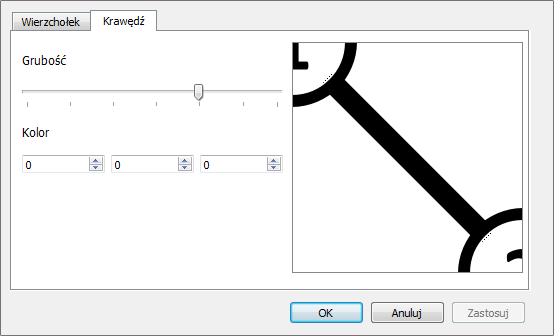
\includegraphics[width=0.9\linewidth]{./img/spec_zew04_2.png}
		\label{fig:grafConfig2}
		\caption{Konfiguracja łuków}
	\end{subfigure}
	\caption{Możliwe zmiany w wyglądzie sieci}
	\label{fig:grafConfig}
\end{figure}
Oba okienka umożliwiają zmianę koloru i rozmiaru, w przypadku wierzchołka możliwa jest ponadto kontrola nad grubością obrysu oraz jego koloru. Kliknięcie przycisku \textit{OK} lub \textit{Zastosuj} skutkuje zapisaniem konfiguracji i aktualizacją wyglądu. Każda sieć posiada swoją lokalną konfigurację, w przypadku zapisywania jej do pliku, ona również jest zachowywana.
\subsubsection{Operowanie na sieci}
Wybierając narzędzie wskaźnika możliwe jest przesuwanie wierzchołków po polu edycyjnym oraz ich zaznaczanie. Można zaznaczyć wiele wierzchołków i łuk przytrzymując klawisz \keys{\ctrl} lub skorzystać z myszki - wystarczy kliknąć lewym przyciskiem na pustym polu, przytrzymać i przeciągnąć kursor by pojawił się prostokąt zaznaczający elementy sieci. Jeżeli jest wiele zaznaczonych elementów przesunięcie jednego z nich spowoduje przesunięcie wszystkich.\\\indent
Zaznaczenie etykiety łuku, informującej o wartościach przepływu i przepustowości, spowoduje pojawienie się linii przerywanej prowadzącej do środka łuku. Ułatwia to pracę z siecią, gdy łuków i etykiet pojawia się coraz więcej.
\begin{figure}[H]
	\centering
	\begin{subfigure}{0.45\textwidth}
		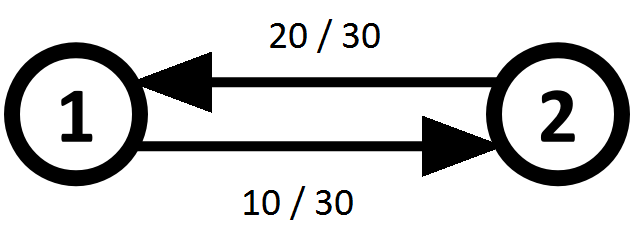
\includegraphics[width=0.9\linewidth]{./img/spec_zew05_1.png}
		\caption{Niezaznaczone etykiety}
		\label{fig:grafSelect1}
	\end{subfigure}
	\begin{subfigure}{0.45\textwidth}
		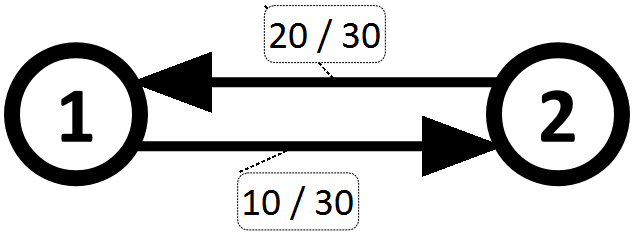
\includegraphics[width=0.9\linewidth]{./img/spec_zew05_2.png}
		\label{fig:grafSelect2}
		\caption{Zaznaczone etykiety}
	\end{subfigure}
	\caption{Przedstawienie linii łączącej etykietę z łukiem}
	\label{fig:grafSelect}
\end{figure}

\subsubsection{Zmiana parametrów łuku}
Nad każdym łukiem znajduje się etykieta, która zawiera informację o wartościach kolejno przepływu i przepustowości oddzielone ukośnikiem. Jeżeli w etykiecie znajduje się jedna liczba, oznacza ona przepustowość. Wówczas wartość przepływu jest zerowa i dla czytelności nie jest wyświetlany. Te dwie wartości można w każdej chwili zmienić klikając dwukrotnie lewym przyciskiem myszy na etykietę. Pojawi się pole edycji, gdzie można wprowadzić nowe wartości. Akceptowane są wyłącznie formaty \lstinline[language=xml]|<liczba>| oraz  \lstinline[language=xml]|<liczba> / <liczba>|. Zmianę zatwierdza się kliknięciem myszy. Nowy łańcuch w poprawnym formacie spowoduje aktualizację wartości i etykiety. Wprowadzenie czegokolwiek innego powoduje przywrócenie pierwotnych wartości.
\subsection{Wykonanie algorytmów}
W momencie utworzenia karty z siecią, nowym lub wczytanym z pliku, w lewym dolnym rogu pojawia się lista dostępnych algorytmów, jakie można wykonać w ramach programu: Forda-Fulkersona, Dinica oraz MKM.
\subsubsection{Warunki poprawności sieci}
Aby uruchomić algorytm sieć musi być poprawnie zbudowana, tzn. spełniać następujące założenia:
\begin{itemize}
	\item wierzchołek źródłowy oraz wierzchołek ujściowy muszą być oznaczone, by móc wyznać maksymalny przepływ. W tym celu należy kliknąć prawym przyciskiem myszki na wierzchołkach i wybrać z menu kontekstowego odpowiednio \textit{oznacz jako źródło} oraz \textit{oznacz jako ujście}. Nad wierzchołkiem źródłowym pojawi się etykieta \textit{\textbf{s}}, a nad wierzchołkiem ujściowym etykieta \textit{\textbf{t}}.
	\item Nie może istnieć żaden wierzchołek, inny niż źródło i ujście, przez który nie istnieje droga ze źródła do ujścia. Ma to na celu zapewnić, że w zbudowanym grafie istnieje co najmniej jedna ścieżka ze źródła do ujścia. Wystarczy, że dla każdego wierzchołka będą istniały co najmniej dwa łuki, wchodzący i wychodzący z niego.
	\item Zasada zachowania przepływu nie może zostać złamana. Program nie dopuszcza, żeby łuk mógł mieć większą wartość przepływu niż przepustowość, ale podczas budowania sieci nie można cały czas kontrolować tej zasady. Jest ona sprawdzana dopiero przy próbie uruchomienia algorytmu.
\end{itemize}
Jeżeli któryś z tych warunków nie zostanie spełniony, pojawi się okienko informujące dokładnie o rodzaju błędu oraz w którym miejscu grafu on wystąpił.
\subsubsection{Okno wykonania}
Jeżeli graf został poprawnie zbudowany, po kliknięciu w jeden z algorytmów pojawi się nowe okno w którym zostanie on wykonany.
\begin{figure}[H]
	\centering
	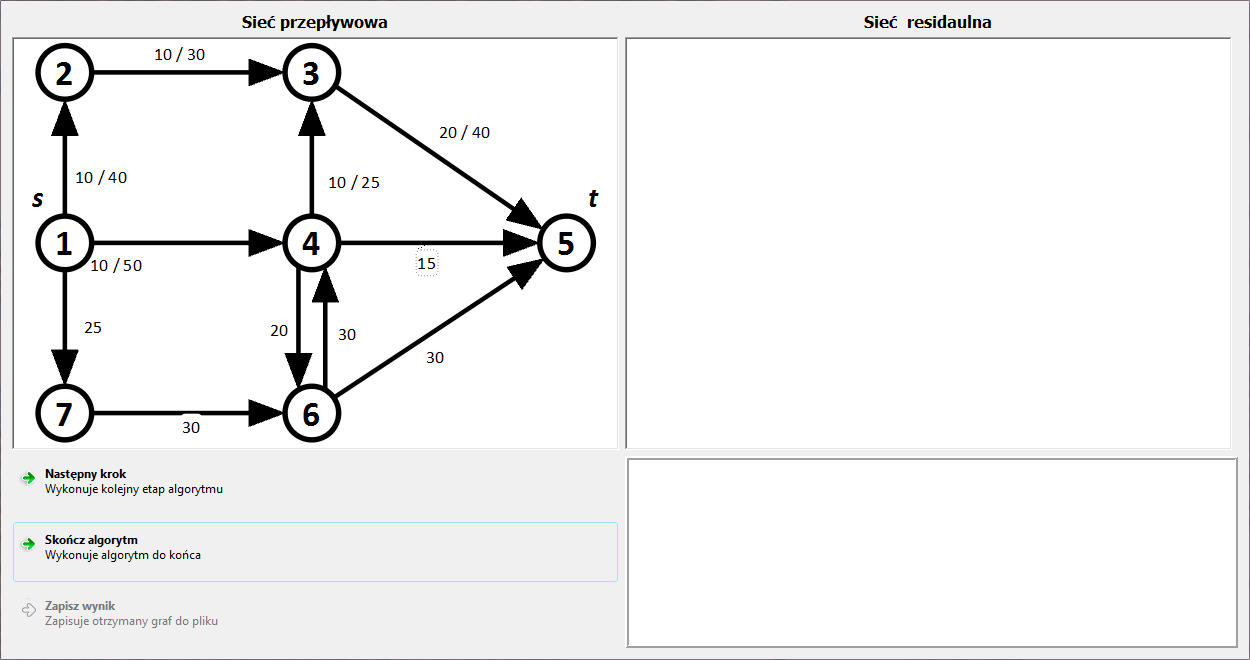
\includegraphics[width=0.85\textwidth]{./img/spec_zew06_1}
	\caption{Okno ilustrujące przebieg algorytmu Forda-Fulkersona}
	\label{fig:algorithmWindowStart}
\end{figure}\noindent
Okno zostało podzielone na 4 obszary:
\begin{itemize}
	\item W górnym lewym rogu znajduje się pierwotna sieć przepływowa, której przepływ zostaje zwiększany wraz z kolejnymi krokami.
	\item W górnym prawym rogu jest podgląd tworzonej sieci residualnej oraz ścieżki powiększającej, jaka została w niej znaleziona. W oknie dla algorytmów Dinica i MKM znajduje się jeszcze dodatkowy, trzeci podgląd, obrazujący zmiany w warstwowej sieci residualnej.
	\item W dolnym lewym rogu znajdują się trzy przyciski:
	\begin{itemize}
		\item \textit{Następny krok}, jego naciśnięcie powoduje wykonanie istotnej instrukcji algorytmu i przedstawienie zaistniałych zmian w podglądach.
		\textit{Skończ algorytm}, realizuje całość zadania, aż maksymalny przepływ zostanie znaleziony. Aplikacja wykonuje wówczas instrukcję \textit{Następny krok} w odstępach równych 0.5 sekundy, aż do zakończenia obliczeń.
		\item \textit{Zapisz wynik}, przycisk staje się uaktywniony po zakończeniu zadania, umożliwia zapisanie sieci ze znalezionym maksymalnym przepływem do pliku XML.
	\end{itemize}
	\item W dolnym prawym rogu znajduje się konsola w której pojawiają się informacje o przebiegu algorytmu. Za każdym razem, gdy instrukcja \textit{Następny krok} zostanie wykonana, w tym polu pojawiają się szczegółowe informacje o utworzonych strukturach, znalezionych przepływach i innych zmianach w sieci.
\end{itemize}
\begin{figure}[H]
	\centering
	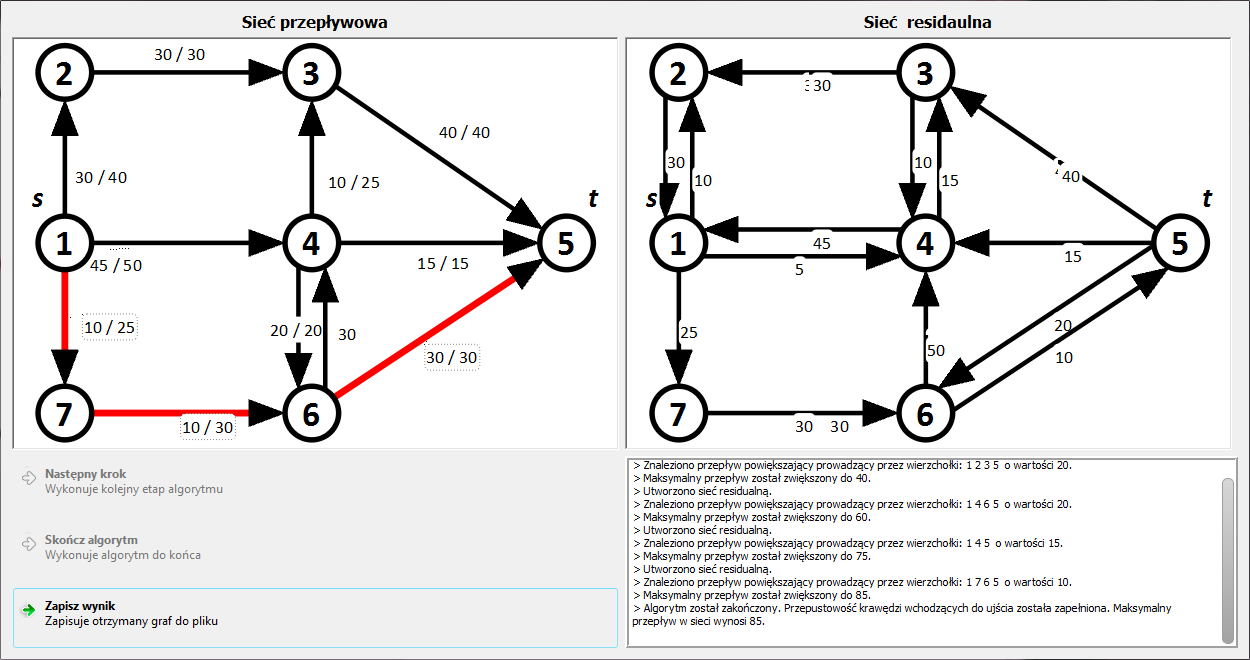
\includegraphics[width=0.85\textwidth]{./img/spec_zew06_5}
	\caption{Okno po zakończeniu wykonywania algorytmu}
	\label{fig:algorithmWindowFinished}
\end{figure}
Przykładowe przedstawienie krok po kroku wyszukiwania maksymalnego przepływu znajduje się w dodatku \ref{add:C}.
\subsection{Otwieranie i zapisywanie}
Aby móc zapisać sieć przepływową do pliku w sesji programu musi być otwarta co najmniej jedna karta. Klikając \keys{\ctrl+S} lub wybierając \menu{Plik > Zapisz jako} można zapisać stan pracy do pliku XML. Program poprosi o wskazanie folderu oraz wpisanie nazwy pliku. Potwierdzenie utworzy nowy plik.
Aby otworzyć plik należy wybrać z paska menu \menu{Plik > Otwórz} lub skorzystać ze skrótu klawiszowego \keys{\ctrl+O}. Program otworzy okno dialogowe i poprosi o wskazanie pliku XML jaki ma otworzyć. Jeżeli ma on poprawny format, sieć przepływowa zostanie wczytana i pokazana w nowej karcie.